\chapter{Results}

In the following sections, the experiment results are presented and analyzed. Further analysis is provided in the following chapter. The sections are separated based on the experiments that had already described in the previous chapters.

\section{Query modeling}

To answer the first research question about the best query model to improve the performance of our baseline, we conduct the query modeling experiment as it is described in the experimental design chapter. Following are the results of this experiment.

\begin{table}[H]
\begin{center}
\caption{System Performance using precision at first five results measure (P@5) of title (T), title and description (T+D), all the fields (T+D+A+C) and attribute and categories (A+C) query models using three retrieval strategies (BM25, LM, TfIdf) and two types of ground truth (editorial and click logs).}

\begin{tabular}{lccccccc}
\toprule
 & \multicolumn{3}{c}{Editorial} & & \multicolumn{3}{c}{Click logs} \\
\midrule
& BM25 & LM & TfIdf &   & BM25 & LM & TfIdf \\
\midrule
T & 0.6560 &  0.5980 & 0.626 &   &         		0.1680 & 0.1660 & 0.1540 \\
T+D & 0.6660 & 0.5880 & 0.6500 &   &    			0.1700 & 0.1680 & \textbf{0.1600} \\
T+D+A+C & \textbf{0.7300} & \textbf{0.6460} & \textbf{0.6860} &   & \textbf{0.1720} & \textbf{0.1700} & 0.1580 \\
A+C & 0.4800 & 0.3400 & 0.4500 &   &     			0.0920 & 0.0900 & \textbf{0.0600} \\
\bottomrule
\end{tabular}
\end{center}
\end{table}

The table represents the precision at five first results from four different query models. First, we are adding fields to our baseline to see if any improvement occurs. The last query model with only attributes and category is an extra query model to compare with and find extra refinements.

As you can see in the results with the editorial evaluation, adding the description to our baseline shows an improvement on precision using BM25 and TfIdf, except LM that shows a minor decrease. Adding the attributes and category gives a boost to all retrieval strategies. However, precision of query model with attributes and category is than our baseline.

The results using the click logs evaluation indicate a slight increase in the precision when the description is used in the query models. Also, adding the attributes and category, shows a small increase but not on TfIdf. However, the attributes and category alone in the query model are not performing better than the baseline.

The results verify our initial assumption that adding extra information on the title query model can improve the performance. We can give an initial answer before further analysis to the first research question that using all the fields on the query model indicates the highest precision thus is the best one of the available query models.


\section{Retrieval modeling}

Second research question that we are answering is about the best retrieval method from the three available. In the table \ref{table:qmRes}, we are presenting the results of the experiment we conducted.

\begin{table}[H]
\begin{center}
\scriptsize
\caption{
System Performance using precision at first five results measure (P@5) of the retrieval strategies Okapi BM25 (BM25), TfIdf, LM and title (T), title and description (T+D), all the fields (T+D+A+C) and attribute and categories (A+C) query models two types of ground truth (editorial and click logs).}
\label{table:qmRes}

\begin{tabular}{lccccccccc}
\toprule
 & \multicolumn{4}{c}{Editorial} & &\multicolumn{4}{c}{Click logs} \\
\midrule
& T & T+D & T+D+A+C & A+C &   & T & T+D & T+D+A+C & A+C \\
\midrule
BM25 & \textbf{0.6560} & \textbf{0.6660} & \textbf{0.7300} & \textbf{0.4800} &   &\textbf{0.1680} & \textbf{0.1700} & \textbf{0.1720} & \textbf{0.0920} \\
LM & 0.5980 & 0.5880 & 0.6460 & 0.3400 &   & 0.1660 & 0.1680 & 0.1700 & 0.0900 \\
TfIdf & 0.626 & 0.6500 & 0.6860 & 0.4500 &   & 0.1540 & 0.1600 & 0.1700 & 0.0600 \\
\bottomrule
\end{tabular}
\end{center}
\end{table}



The table represents the precision at five first results of the three retrieval strategies using four different query models. As you can see on the results with editorial evaluation, LM has the smallest precision in a comparison with the other two. BM25 is performing better in both editorial and click logs evaluation. Furthermore, in results with click logs evaluation in one query model LM and TfIdf have the same precision. However, in attributes and category query models TfIdf has lower precision than LM.

Provided with the previous results, we can verify that Okapi BM25 is the retrieval strategy which performs better than the other two.


\section{LDF}

Different late data fusion techniques used to answer the third research question about improving the performance of the individual systems using late these techniques.

\begin{table}[H]
\begin{center}
\footnotesize
\caption{System Performance using precision at first five results measure (P@5) of late data fusion methods (combMAX, combMIN, combSUM, combMNZ, combANZ, WcombSUM, WcomMNZ, WcombWW) and the best individual system using two types of ground truth (editorial and click logs).}
\begin{tabular}{lcr}
\midrule
  & Editorial & Clicks logs\\
 \midrule
	combMAX & 0.5400 & 0.1280\\
	combMIN & 0.0760 & 0.0020 \\
	combSUM & 0.6160 & 0.1720 \\
	combMNZ & 0.6460 & 0.1720 \\
	combANZ & 0.0800 & 0.0020 \\
	WcombSUM & 0.6140 & \textbf{0.1740} \\
	WcombMNZ & 0.6360 & \textbf{0.1740} \\
	WcombWW & 0.6320 & \textbf{0.1740} \\
	Best Individual & \textbf{0.7300} & 0.1720 \\
\bottomrule
\end{tabular}
\end{center}
\end{table}






The table represents all the late fusion methods we use to answer the third research question in a comparison with the individual best system. The most important observation of this table is that none of the fused systems is performing better than the individual one using the editorial evaluation.

On the results with the editorial evaluation, the compMNZ is performing better than the rest of the fused systems. The rest of the fused systems have small differences in the precision except of the combMIN and combANZ that have very low precision.

On the results with click logs evaluation, the weighted fused systems have better precision than the rest. Then, a slight decrease in precision is seen on combMNZ and combMAX and a bigger decrease on combMAX. Same as editorial evaluation, the combANZ and combMIN have the lowest precision.


\section{Diversification}

Performance of the different diversification approaches we use on the diversification experiment are presented to graphs of figure 5.1 to answer the following research questions:

The research questions we aim to answer are the following:
\begin{enumerate}
\item Are the results of diversification affected if only the similarity with the previous displayed classified is taken into account?
\item Are the results of diversification affected if the average similarity of previous displayed docs is taken into account?
\item Are the results of diversification affected if only the similarity with the previous four displayed classifieds is taken into account?
\end{enumerate}

% Overall Accuracy
\begin{figure}[H]
\centering
\begin{minipage}{.5\textwidth}
	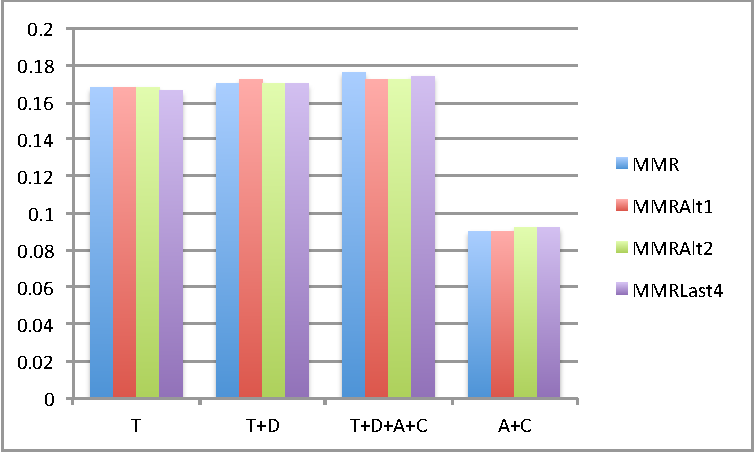
\includegraphics[width=.9\linewidth]{../images/MMRMethodsP@5.pdf}
	\subcaption{Click logs}
	\label{fig:acc-ns}
\end{minipage}%
\begin{minipage}{.5\textwidth}
	\centering
	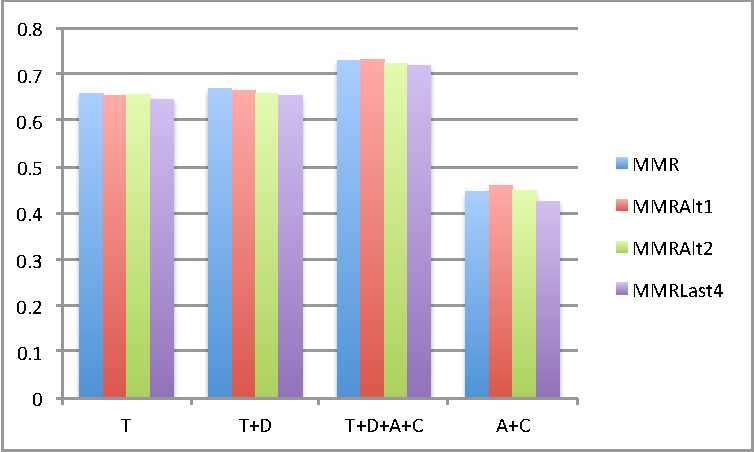
\includegraphics[width=.9\linewidth]{../images/MMRMethodsP@5Relevance.pdf}
	\subcaption{Editorial}
	\label{fig:acc-ns}
\end{minipage}%
\caption{Bar graphs with the system performance (P@5) of diversification methods MMR, MMRAlt1, MMRAlt2, MMRLast4 using title (T), title and description (T+D), all the fields (T+D+A+C) and attribute and categories (A+C) query models and two types of ground truth (editorial and click logs).
}
\end{figure}


In the previous graphs, the precision in five first results for the alternative diversification methods using four different query models is presented. In both graphs the trends are almost the same thus none of the systems performs better than the others. So, as a first and fast answer in the diversification research questions (four, five and six) is that none of them performs better than the MMR method proposed on \cite{CarbonellGoldstein}.


\section{Fused diversified results}

Final research question on the improvement fusion of diversified systems improve the performance of the not diversified systems?

\begin{table}[H]
\begin{center}
\footnotesize
\caption{System Performance using precision at first five results measure (P@5) of late data fusion methods (combMAX, combMIN, combSUM, combMNZ, combANZ, WcombSUM, WcombMNZ, WcombWW) of fused system and fused diversified system using two types of ground truth (editorial and click logs).}
\begin{tabular}{lccccc}
\toprule
 & \multicolumn{2}{c}{Editorial} & & \multicolumn{2}{c}{Click logs} \\
\midrule
 & Fused diversified & Fused not diversified &   & Fused diversified & Fused not diversified \\
 \midrule
	combMAX & \textbf{0.7320} & 0.5400 &   & 0.1700 & 0.1280 \\
	combMIN & 0.0800 & 0.0760 &   & 0.0020 & 0.0020 \\
	combSUM & 0.6700 & 0.6160 &   & 0.1720 & 0.1720 \\
	combMNZ & 0.6700 & 0.6460 &   & 0.1720 & 0.1720 \\
	combANZ & 0.0940 & 0.0800 &   & 0.0040 & 0.0020 \\
	WcombSUM & 0.6620 & 0.6140 &   & 0.1720 & \textbf{0.1740} \\
	WcombMNZ & 0.6560 & 0.6360 &   & 0.1720 & \textbf{0.1740} \\
	WcombWW & 0.6560 & 0.6320 &   & 0.1720 & \textbf{0.1740} \\
\bottomrule
\end{tabular}
\end{center}
\end{table}

The previous two tables represent the comparison of the results of fused diversified systems versus the fusion of individual systems with both click logs and editorial evaluation.

Using the click logs evaluation, we can't see a big difference except of the 0.5 increase on combMAX when the system is diversified.

Using the relevance feedback, we can see a small improvement in precision in all the systems. Also, the biggest difference is in the combMAX which has an increase of 0.19. The smallest increase we have in this table is the combANZ which is 0.014.

All in all, using the editorial evaluation we can verify and answer to the seventh research question that the fused diversified systems perform better than the fused not diversified systems. Using the click log evaluation, we can not give the same answer cause the results in the table don't show any big improvement.


Research questions had already answered with the results of this chapter. A deeper analysis and assumptions about the reasons we have these results are provided in the next chapter.
